% This is paper draft
% edited by Haoruo Peng
% Date: 2013.1.6
\documentclass{llncs}
\usepackage{llncsdoc}
\usepackage{amsmath, amssymb}
\usepackage{color}
\usepackage{graphicx}

\newcommand{\bw}{\mathbf{w}}
\newcommand{\bwep}{\mathbf{w}^{\varepsilon}}
\newcommand{\bwfly}{\tilde{\mathbf{w}}}
\newcommand{\bwavg}{\mathbf{wavg}}
\newcommand{\bu}{\mathbf{u}}
\newcommand{\buprev}{\mathbf{uprev}}
\newcommand{\bp}{\mathbf{p}}
\newcommand{\bq}{\mathbf{q}}
\newcommand{\bxi}{\mathbf{\xi}}
\newcommand{\dotwxb}{{\mathbf{w}}^{\mathbf{T}}\mathbf{x}_{i}+b}
\newcommand{\sumt}{\sum_{t=1}^{T} }
\newcommand{\lc}{\left(}
\newcommand{\rc}{\right)}
\newcommand{\li}{\lc i\rc}
\newcommand{\lj}{\lc j\rc}
\newcommand{\tspace}{\hspace*{2em}}
\newcommand{\tspaces}{\hspace*{1.5em}}
\newcommand{\comment}{\textcolor{red}}
\newcommand{\ti}[1]{\tilde{#1}}
\newcommand{\indep}{{\;\bot\!\!\!\!\!\!\bot\;}}

\def\A{{\bf A}}
\def\a{{\bf a}}
\def\B{{\bf B}}
\def\C{{\bf C}}
\def\c{{\bf c}}
\def\D{{\bf D}}
\def\d{{\bf d}}
\def\E{{\bf E}}
\def\e{{\bf e}}
\def\f{{\bf f}}
\def\K{{\bf K}}
\def\H{{\bf H}}
\def\G{{\bf G}}
\def\I{{\bf I}}
\def\R{{\bf R}}
\def\X{{\bf X}}
\def\Y{{\bf Y}}
\def\Q{{\bf Q}}
\def\s{{\bf s}}
\def\S{{\bf S}}
\def\x{{\bf x}}
\def\y{{\bf y}}
\def\z{{\bf z}}
\def\Z{{\bf Z}}
\def\M{{\bf M}}
\def\m{{\bf m}}
\def\n{{\bf n}}
\def\U{{\bf U}}
\def\u{{\bf u}}
\def\V{{\bf V}}
\def\v{{\bf v}}
\def\W{{\bf W}}
\def\w{{\bf w}}
\def\0{{\bf 0}}
\def\1{{\bf 1}}

\def\AM{{\mathcal A}}
\def\FM{{\mathcal F}}
\def\TM{{\mathcal T}}
\def\UM{{\mathcal U}}
\def\XM{{\mathcal X}}
\def\YM{{\mathcal Y}}
\def\NM{{\mathcal N}}
\def\OM{{\mathcal O}}
\def\IM{{\mathcal I}}
\def\GM{{\mathcal G}}
\def\RB{{\mathbb R}}

\def\tx{\tilde{\bf x}}
\def\ty{\tilde{\bf y}}
\def\tz{\tilde{\bf z}}
\def\hd{\hat{d}}
\def\HD{\hat{\bf D}}
\def\hx{\hat{\bf x}}

\def\alp{\mbox{\boldmath$\alpha$\unboldmath}}
\def\bet{\mbox{\boldmath$\beta$\unboldmath}}
\def\epsi{\mbox{\boldmath$\epsilon$\unboldmath}}
\def\etab{\mbox{\boldmath$\eta$\unboldmath}}
\def\ph{\mbox{\boldmath$\phi$\unboldmath}}
\def\pii{\mbox{\boldmath$\pi$\unboldmath}}
\def\Ph{\mbox{\boldmath$\Phi$\unboldmath}}
\def\Ps{\mbox{\boldmath$\Psi$\unboldmath}}
\def\tha{\mbox{\boldmath$\theta$\unboldmath}}
\def\Tha{\mbox{\boldmath$\Theta$\unboldmath}}
\def\muu{\mbox{\boldmath$\mu$\unboldmath}}
\def\Si{\mbox{\boldmath$\Sigma$\unboldmath}}
\def\Gam{\mbox{\boldmath$\Gamma$\unboldmath}}
\def\Lam{\mbox{\boldmath$\Lambda$\unboldmath}}
\def\De{\mbox{\boldmath$\Delta$\unboldmath}}
\def\vps{\mbox{\boldmath$\varepsilon$\unboldmath}}

\def\Ncal{\mathcal{N}}
\def\argmax{\mathop{\rm argmax}}
\def\argmin{\mathop{\rm argmin}}

\def\sgn{\mathrm{sgn}}
\def\tr{\mathrm{tr}}
\def\rk{\mathrm{rank}}
\def\diag{\mathsf{diag}}
\def\vect{\mathsf{vec}}
\def\etal{{\em et al.\/}\,}

%\newtheorem{theorem}{Theorem}
%\newtheorem{lemma}{Lemma}
%\newtheorem{definition}{Definition}
%\newtheorem{proposition}{Proposition}
%\newtheorem{corollary}{Corollary}
%\newtheorem{example}{Example}

\begin{document}
\mainmatter  % start of an individual contribution

% first the title is needed
\title{Parallel Sublinear Algorithms for Penalized Logistic Regression in Massive Datasets}

% a short form should be given in case it is too long for the running head
\titlerunning{Parallel Sublinear Algorithms for Penalized Logistic Regression in Massive Datasets}

%
%\author{Haoruo Peng\inst{1, 2}  \and Zhengyu Wang\inst{1, 3}  \and Edward Y. Chang\inst{1} \and Zhihua Zhang\inst{1, 4}}
%
%\authorrunning{Haoruo Peng \and Zhengyu Wang \and Edward Y. Chang \and Zhihua Zhang}
% (feature abused for this document to repeat the title also on left hand pages)

%\institute %
%{
%\inst{}
%HTC Research, Beijing, China 100084 \\
%\and
%\inst{}
%Department of Computer Science and Technology\\
%Tsinghua University, Beijing, China 100084
%\and
%\inst{}
%Institute for Interdisciplinary Information Sciences\\
%Tsinghua University, Beijing, China 100084
%\and
%\inst{}
%College of Computer Science and Technology \\
%Zhejiang University, Zhejiang, China 310027 \\
%\email{penghaoruo@hotmail.com wangsincos@163.com eyuchang@gmail.com georgezhou@google.com zhzhang@cs.zju.edu.cn}
%}
%
%\toctitle{Lecture Notes in Computer Science}
%\tocauthor{Authors' Instructions}
\maketitle

\begin{abstract}
Penalized logistic regression (PLR) is a widely used supervised learning model.
In this paper, we present a parallel implementation of sublinear algorithms for PLR to efficiently improve scalability.
We develop concrete parallel algorithms for PLR with $\ell_2$-norm and $\ell_1$-norm penalties, respectively with MapReduce.
Due to the intrinsic random nature of the proposed parallel algorithms, they can provide fault recovery for lengthy distributed computations.
They also enjoy the benefits of sublinear dependency on both the volume and dimensionality of training data, and can be widely applied to many large real-world datasets.
We have released MapReduce-PSUBPLR to open source at http://code.google.com/p/psubplr.
\end{abstract}

\section{Introduction} \label{sec:int}

The penalized logistic regression (PLR) model~\cite{HastieBook:SL} plays an important role in machine learning and data mining.
The model serves for classification problems, and enjoys a substantial body of supporting theories and algorithms.
PLR is competitive with the support vector machines (SVMs) \cite{Vapnik:1998}, because it has both high accuracy and  interpretability (PLR can directly estimate a conditional class probability).

Recently, large-scale applications have emerged from many modern massive datasets.
A key characteristic of these applications is that the size of their training data is very large and data dimensionality is very high.
For example, in medical diagnostic applications~\cite{tsumoto2004mining}, both doctors and patients would like to take the advantage of millions of records over hundreds of attributes. More evidently, search engines on texts or multimedia data must handle data volume in the billion scale and each data instance is characterized by a feature space of thousands of dimensions~\cite{genkin2007large}.
Large data volume and high data dimensionality pose computational challenges to machine learning problems.

We tackle these challenges via stochastic approximation approaches.
Stochastic approximation methods, such as stochastic gradient descent~\cite{zhang2004solving} and stochastic dual averaging~\cite{xiao2010dual}, obtain optimal generalization guarantees
with only a single pass or a small number of passes over the data.
Therefore, they can achieve a desired generalization  with runtime linear to the dataset size.
We further speed up the runtime, and propose sublinear algorithms for PLR via the use of stochastic approximation idea.
Our algorithms work at the same level of performance with traditional learning methods for PLR, but require much shorter running time.
Our methods access a single feature of training vectors instead of entire training vectors at each iteration.
This {\em sampling} approach brings much improved computational efficiency by eliminating a large number of vector multiplication operations.
By devising clever randomized algorithms, we can also enjoy the benefits of taking less number of iterations and hence accessing less number of features.
Such reduction in accessing features can substantially reduce running time as pointed out by~\cite{hazanbeating}.

Our algorithms can be easily applied to distributed storage systems~\cite{hogan1990livermore} with parallel updates on all instances.
We can achieve good scalability in massive datasets with a MapReduce implementation.
	
The rest of the paper is organized as follows:
Section~\ref{sec:rew} discusses some related work.
In Section~\ref{sec:plr}, we review the penalized logistic regression model along with the sublinear algorithms.
In Section~\ref{sec:framework}, we present the parallel framework of our sublinear algorithms for PLR.
In Section~\ref{sec:alg}, we depict detailed algorithms and analysis.
Section~\ref{sec:experiment} describes the datasets and the baseline of our experiments and presents the experimental results.
Finally, we offer our concluding remarks in Section~\ref{sec:concl}.

\section{Related Work} \label{sec:rew}
There are many existing techniques that address logistic regression with $\ell_1$-penalty in the literature.

The \textit{Reduced Memory Multi-pass} (RMMP) algorithm, proposed by Balakrishnan and Madigan \cite{balakrishnan2008algorithms}, is one of the most accurate and fastest convergent algorithms.
RMMP trains sparse linear classifiers on high-dimensional datasets in a multi-pass manner.
However, this algorithm has computational complexity and memory requirements that make learning on large-scale datasets extremely computational expensive.
The central idea of the work is a straightforward quadratic approximation to the likelihood function.
When the dimensionality of the data gets large, the cost of many vector-vector multiplication operations increases significantly.
Also, the quadratic approximation is added together for all instances in each iteration, and such computation inevitably requires global reduction in a distributed storage system.

The \textit{Hybrid Iterative Shrinkage} (HIS) algorithm, proposed by Shi et al. \cite{shi2008fast}, is also computationally efficient without loss of classification accuracy.
This algorithm includes a fixed point continuation phase and an interior point phase.
The first phase is based completely on memory efficient operations such as matrix-vector multiplications, while the second phase is based on a truncated Newton's method.
Thus, HIS is in the scope and constraints of traditional way of solving the optimization problem.
As RMMP has relatively better scalability and performance, we choose to use RMMP instead of HIS as our baseline for the empirical comparison in this paper.

Recently, Clarkson et al. \cite{clarkson2010sublinear} proposed a new method by taking advantage of randomized algorithms.
They presented sublinear-time approximation algorithms for optimization problems arising in machine learning, such as linear classifiers and minimum enclosing balls.
The algorithm uses a combination of a novel sampling techniques and a new multiplicative update algorithm. They also proved lower bounds which show the running times to be nearly optimal on the unit-cost RAM model.

Hazan et al. \cite{hazanbeating} exploited sublinear approximation approach to the linear SVM with $\ell_2$-penalty, from which we were inspired and borrowed some of the ideas (We generally refer to them as the ETN framework in Section~\ref{sec:framework}).
Later on, Cotter et al. \cite{cotter2012kernelized} extended the work to kernelized SVM cases.
In \cite{hazan2011optimal}, Hazan et al. applied the sublinear approximation approach for solving ridge ($\ell_2$-regularized) and lasso ($\ell_1$-regularized) linear regression.
Garber and Hazan \cite{garberapproximating} developed the method in semidenfinite programming (SDP).

In this paper, we mainly target the size of the training data at the Gigabytes level. These datasets require us to develop machine learning algorithms towards a more efficient and more parallelized end. In the Hadoop programming environment, researchers have already done much work to cater for the needs of massive datasets.

Early work like PSVM (\textit{Parallel Support Vector Machines}) \cite{chang2007psvm} employed an approximation matrix decomposition method based on row selections to reduce the memory when running the algorithm. It can then increase the number of participated parallel computation nodes to several hundreds. Later, the work of PLDA (\textit{Parallel Latent Dirichlet Allocation}) \cite{wang2009plda} further improve the computational efficiency through the use of sampling methods. The proposed parallel algorithm in Hadoop is robust, for it has fault tolerance of machines, taking the advantage of Hadoop. Recently, the work by Dean et al. \cite{dean2007largescale} showed that the advantage of parallelization is fully taken in deep learning algorithms. It pushed the limits of parallel computational nodes to a hundred-million level, and in the meantime, achieved a best learning performance ever. Besides Hadoop, there are many other trials on parallelization in machine learning. GraphLab \cite{kyrola2012graphchi}, a recent developed tool in CMU (\textit{Carnegie Mellon University})for large-scale machine learning, tried to tackle with intrinsic problems of Hadoop when applied to machine leaning algorithms. However, the original design purpose is to improve efficiency in a single-machine multi-core situation, which is a drawback in a distributed system.

\section{Learning Algorithms for Penalized Logistic Regression Models} \label{sec:plr}

Logistic regression is a widely used method for solving classification problems.
In this paper, we are mainly concerned with the binary classification problem.  	
Suppose that we are given a set of training data $\XM=\{(\x_i, y_i): i=1, \ldots, n\}$ where $\x_i \in \RB^d$ are input samples and $y_i \in \{-1, 1\}$ are the corresponding labels.
For simplicity, we let $\X=[{\x}_{1}, {\x}_{2}, \ldots, {\x}_n]^{T}$ and $\y=(y_1, y_2, \ldots, y_n)^T$.
In the logistic regression model, the expected value of $y_i$ is given by
\[
P(y_i|\x_i)= \frac{1}{1+ \exp(- y_i(\x_i^T \w + b))} \triangleq g_i(y_i),
\]
where $\w=(w_1, \ldots, w_d)^T \in \RB^d$ is a regression vector and $b\in \RB$ is an offset term.

\subsection{Penalized Logistic Regression Models}
	
We assume that $\w$ follows a Gaussian distribution with mean $\0$ and covariance matrix $\lambda \I_d$ where $\I_d$ is the $d{\times}d$ identity matrix, i.e. $\w \thicksim N(\0, \lambda \I_d)$.
In this case, we can formulate the optimization problem as
\begin{equation} \label{eqn:4}
	\max_{\bw ,b} \; \Big\{F(\w, b| \XM) - \frac{\lambda}{2}  \|\bw\|_2^{2} \Big\}.
\end{equation}
(\ref{eqn:4}) shows us that the problem reduces to an optimization problem with an $\ell_2$-penalty.
	
In another case, we impose a Laplace prior for $\w$, whose density is given by
\[	
\log\,p\lc\bw \rc=d\,\log\frac{\gamma}{2}-\gamma{\|\bw\|}_{1}.
\]
With this prior, we formulate an optimization problem with the $\ell_1$-penalty. $\ell_1$-penalty logistic regression can serve for both classification and feature selection simultaneously.
\begin{equation} \label{eqn:5}
	\max_{\bw ,b} \;  \big\{F(\w, b|\XM)- \gamma{\|\bw \|}_{1}\big\}.	
\end{equation}

\subsection{Sublinear Algorithms}

The framework of sublinear algorithms is a hybrid method to handle hard margin and soft margin separately and simultaneously.
It enjoys the property of fast convergence for both hard margin and soft margin.

Each iteration of the method works in two steps.
The first one is the \textit{stochastic primal update}:
\begin{enumerate}
\item[{(1)}] \; An instance $i\in \{1,\ldots, n\}$ is chosen according to a probability vector $\bp$;
\item[{(2)}] \; The primal variable $\bw$ is updated according to the derivative of $f_i(\bw,b)$ and the soft margin, via an online update with regret.
\end{enumerate}

The second one is the \textit{stochastic dual update}:
\begin{enumerate}
\item[{(1)}] \; A stochastic estimate of $f_i(\bw,b)$ plus the soft margin is obtained, which can be computed in $O(1)$ time per term;
\item[{(2)}] \; The probability vector $\bp$ is updated based on the above computed terms by using the \textit{Multiplicative Updates} (MW) framework~\cite{arora2005multiplicative} for online optimization over the simplex.
\end{enumerate}

We use the following notations in our algorithms and analysis.

$clip\lc \cdot \rc$ is a projection function defined as follows:
	\[
	clip\lc a,b \rc \triangleq \max \lc \min \lc a,b \rc ,-b\rc \,\,\,\,\,\, a,b \in \mathbb{R}.
	\]

$\sgn \lc \cdot \rc$ is the sign function; namely,
	
	\[
	\sgn \lc x \rc =
		\begin{cases}
 		+1 & \text{ if } x>0  \\
 		0  & \text{ if } x=0  \\
 		-1 & \text{ if } x<0.
		\end{cases}
	\]

$g\lc \cdot \rc$ is the logistic function; namely,
	\[
	g \lc x \rc=\frac{1}{1+e^{-x}}
	\]

We let $\Lambda$ be the $\mathbb{R}_{n}$ Euclidean space which meets the following conditions:
	\[
	\Lambda=\left\{ \bxi\in\mathbb{R}_{n} \, | \, \forall i, \, 0\leq{\xi}_{i}\leq 2, \, {\|\xi \|}_{1}\leq \nu n  \right
	\}.
	\]

\subsection{Sequential Sublinear Algorithm for $\ell_2$-Penalty Logistic Regression} \label{sec:l2alg}
	
	\begin{table} [ht]
	\begin{tabular}{l}
	\hline\noalign{\smallskip}
	\textbf{Algorithm 1} SLLR-L2 \\
	\noalign{\smallskip}
	\hline
	\noalign{\smallskip}
		1:    Input: $\varepsilon>0, 0\leq\nu\leq1, X\in\mathbb{R}^{n\times d}, Y\in\mathbb{R}^{n} $ \\
		2:    Let $T\leftarrow{1000}^{2}{\varepsilon}^{-2}\log n, \eta\leftarrow\sqrt{\log\lc n\rc/T}$ \\
		3:    \tspace ${\mathbf{u}}_{0}\leftarrow{\mathbf{0}}_{d},{\bw}_{1}\leftarrow{\mathbf{0}}_{d},{\mathbf{\bq}}_{1}\leftarrow{\mathbf{1}}_{n},{b}_{1}\leftarrow 0$\\
		4:    \textbf{for} $t=1$ to $T$ \textbf{do} \\
		5:    \tspace ${\bp}_{t}\leftarrow{\bq}_{t}/{\|{\bq}_{t}\|}_{1}$ \\
		6:    \tspace Choose ${i}_{t}\leftarrow i$ with probability $\bp(i)$ \\
		7:    \tspace Let $coef={y}_{{i}_{t}}g\lc-{y}_{{i}_{t}}\lc {{\bw}_{t}}^{T}{\mathbf{x}}_{i_t}+{b}_{t} \rc\rc$ \\
		8:    \tspace Let ${\bu}_{t}\leftarrow {\bu}_{t-1}+\frac{coef}{\sqrt{2T}}{\mathbf{x}}_{{i}_{t}}$ \\
		9:    \tspace\tspace ${\bxi}_{t}\leftarrow \argmax_{\bxi\in \Lambda}\lc{{\bp}_{t}}^{T}\bxi\rc$ \\
		10:   \tspace\hspace*{1.2em} ${b}_{t}\leftarrow \sgn\lc {{\bp}_{t}}^{T}\mathbf{y}\rc$ \\
		11:   \tspace ${\bw}_{t}\leftarrow {\bu}_{t}/\max \left\{1,\|{\bu}_{t}\|_2 \right\}$ \\
		12:   \tspace Choose ${j}_{t}\leftarrow j$ with probability ${{\bw}_{t}\lj}^{2}/{\|{\bw}_{t}\|_2}^{2} $ \\
		13:   \tspace \textbf{for} $i=1$ to $n$ \textbf{do} \\
		14:   \tspace\tspace $\sigma \leftarrow \mathbf{x}_{i} \lc {j}_{t}\rc{\|{\bw}_{t}\|_2}^{2}/{\bw}_{t}\lc {j}_{t} \rc+{\bxi}_{t}\li+{y}_{i}{b}_{t}$ \\
		15:   \tspace\tspace $\hat{\sigma} \leftarrow clip\lc \sigma,1/\eta \rc$ \\
		16:   \tspace\tspace ${\bq}_{t+1}\li \leftarrow {\bq}_{t}\li\lc 1-\eta\hat{\sigma} + {\eta}^{2}{\hat{\sigma}}^{2} \rc$ \\
		17:   \tspace \textbf{end for} \\
		18:   \textbf{end for} \\
		19:   Output: $\bar{\bw}=\frac{1}{T}\sum_{t}{\bw}_{t},\bar{b}=\frac{1}{T}\sum_{t}{b}_{t}$ \\
	\hline
	\end{tabular} 	
	\label{alg:1}
	\end{table}

    In Algorithm~1, we give the sublinear approximation procedure for $\ell_2$-penalty logistic regression.	

\subsection{Sequential Sublinear Algorithm for $\ell_1$-Penalty Logistic Regression}
	
    \begin{table}[ht]
	\begin{tabular}{l}
	\hline\noalign{\smallskip}
	\textbf{Algorithm 2} SLLR-L1 \\
	\noalign{\smallskip}
	\hline
	\noalign{\smallskip}
		1:    Input: $\varepsilon>0, \gamma>0, X\in\mathbb{R}^{n\times d}, Y\in\mathbb{R}^{n}$ \\
		2:    Let $T\leftarrow{1000}^{2}{\varepsilon}^{-2}\log n, \eta\leftarrow\sqrt{\log\lc n\rc/T}$ \\
		3:    \tspace ${\mathbf{u}}_{0}\leftarrow{\mathbf{0}}_{d},{\bwavg}_{0}\leftarrow{\mathbf{0}}_{d},{\mathbf{\bq}}_{1}\leftarrow{\mathbf{1}}_{n},{b}_{1}\leftarrow 0$\\
		4:    \textbf{for} $t=1$ to $T$ \textbf{do} \\
		5:    \tspace ${\bp}_{t}\leftarrow{\bq}_{t}/{\|{\bq}_{t}\|}_{1}$ \\
		6:	  \tspace $\buprev_t\leftarrow\bu_{t-1}$ \\
		7:    \tspace Choose ${i}_{t}\leftarrow i$ with probability $\bp(i)$ \\
		8:    \tspace Let $coef={y}_{{i}_{t}}g\lc-{y}_{{i}_{t}}\lc {{\bwavg}_{t-1}}^{T}{\mathbf{x}}_{i_t}+{b}_{t} \rc\rc$ \\
		9:    \tspace Let ${\bu}_{t}\leftarrow {\bu}_{t-1}+\frac{coef}{\sqrt{2T}}{\mathbf{x}}_{{i}_{t}}$ \\
		10:   \tspaces\tspace ${b}_{t}\leftarrow \sgn\lc {{\bp}_{t}}^{T}\mathbf{y}\rc$ \\
		11:   \tspaces \textbf{for} $j=1$ to $d$ \textbf{do} \\
		12:   \tspaces\tspace \textbf{if} $\buprev_t\lj>0$ \textbf{and} $\bu_t\lj>0$ \\
		13:	  \tspaces\tspace\tspace $\bu_t\lj=\max \lc \bu_t\lj-\gamma ,0 \rc$ \\
		14:	  \tspaces\tspace \textbf{if} $\buprev_t\lj<0$ \textbf{and} $\bu_t\lj<0$ \\
		15:   \tspaces\tspace\tspace $\bu_t\lj=\min \lc \bu_t\lj+\gamma ,0 \rc$ \\
		16:   \tspaces \textbf{end for} \\
		17:   \tspaces ${\bw}_{t}\leftarrow {\bu}_{t}/\max \left\{1,\|{\bu}_{t}\|_2 \right\}$ \\
		18:   \tspaces ${\bwavg}_{t}\leftarrow \frac{t-1}{t}{\bwavg}_{t-1}+\frac{1}{t}\bw_t$ \\
		19:   \tspaces Choose ${j}_{t}\leftarrow j$ with probability ${{\bw}_{t}\lj}^{2}/{\|{\bw}_{t}\|_2}^{2} $ \\
		20:   \tspaces \textbf{for} $i=1$ to $n$ \textbf{do} \\
		21:   \tspaces\tspace $\sigma \leftarrow \mathbf{x}_{i} \lc {j}_{t}\rc{\|{\bw}_{t}\|_2}^{2}/{\bw}_{t}\lc {j}_{t} \rc+{y}_{i}{b}_{t}$ \\
		22:   \tspaces\tspace $\hat{\sigma} \leftarrow clip\lc \sigma,1/\eta \rc$ \\
		23:   \tspaces\tspace ${\bq}_{t+1}\li \leftarrow {\bq}_{t}\li\lc 1-\eta\hat{\sigma} + {\eta}^{2}{\hat{\sigma}}^{2} \rc$ \\
		24:   \tspaces \textbf{end for} \\
		25:   \textbf{end for} \\
		26:   Output: $\bwavg_t,\bar{b}=\frac{1}{T}\sum_{t}{b}_{t}$ \\
	\hline
	\end{tabular}
	\end{table}

\section{Parallel Framework of PSUBPLR} \label{sec:framework}
	
In this section, we develop an approach to solve sublinear learning for penalized logistic regression using the architecture of MapReduce.

	\begin{table}[ht]
	\begin{tabular}{l}
	\hline\noalign{\smallskip}
	\textbf{Procedure} PSUBPLR \\
	\noalign{\smallskip}
	\hline
	\noalign{\smallskip}
        Input parameters: $\varepsilon, X, Y, n, d$ \\
        \hspace*{7.8em} $\nu$ // \textsl{(for $\ell_2$-penalty)} \\
        \hspace*{7.8em} $\gamma$ // \textsl{(for $\ell_1$-penalty)} \\
        Let $T\leftarrow\frac{1}{n}{1000}^{2}{\varepsilon}^{-2}\log n, \eta\leftarrow\sqrt{\log\lc n\rc/T}$ \\
        \hspace*{1.5em} ${\bw}_{1}\leftarrow{\mathbf{0}}_{d}, {\mathbf{\bp}}_{1}\leftarrow{\mathbf{1}}_{n}, {b}_{1}\leftarrow 0$\\
		\textbf{for} $t=1$ to $T$ \textbf{do} \\
        \tspace HDFS-File("paraw") $\leftarrow \textit{Write-in-HDFS-File}(\bw_t)$ \\
        \tspace $\textit{add-to-distributed-cache}$(HDFS-File("paraw"))   \\
        \tspace HDFS-File("parap") $\leftarrow \textit{Write-in-HDFS-File}(\bp_t)$ \\
        \tspace $\textit{add-to-distributed-cache}$(HDFS-File("parap"))   \\
		\tspace Primal-MR $\leftarrow$ \textbf{new} \textit{MapReduce-Job}() \\
        \tspace Primal-MR\textit{.configuration.setparameters}($T, n, d, b_t$) \\
        \tspace Primal-MR\textit{.configuration.setOutputFilePath}("sublinear/tmp/primal$t$") \\
        \tspace Primal-MR\textit{.start}() \\ 
        \tspace Primal-MR\textit{.waitForCompletion}() \\
        \tspace ($\bw_{t+1}, b_{t+1}$)$\leftarrow$\textit{PrimalUpdate}($\bw_t, b_t$) \\
        \tspace \textit{soft-thresh-holding}($\bw_{t+1}$) // \textsl{for $\ell_1$-penalty only} \\
        \tspace $j_t \leftarrow \textit{samplingFrom}(d)$ // with probability vector ${{\bw}_{t+1}\lj}^{2}/{\|{\bw}_{t+1}\|_2}^{2}$, for $j\in \{1,\ldots, d\}$ \\
        \tspace HDFS-File("paraw") $\leftarrow \textit{Write-in-HDFS-File}(\bw_{t+1})$ \\
        \tspace $\textit{add-to-distributed-cache}$(HDFS-File("paraw"))   \\
        \tspace Dual-MR $\leftarrow$ \textbf{new} \textit{MapReduce-Job}() \\
        \tspace Dual-MR\textit{.configuration.setparameters}($d, jt, b_{t+1}, \eta$) \\
        \tspace Dual-MR\textit{.configuration.setOutputFilePath}("sublinear/tmp/dual$t$") \\
        \tspace Dual-MR\textit{.start}() \\
        \tspace Dual-MR\textit{.waitForCompletion}() \\
        \tspace $\bp_{t+1}$$\leftarrow$\textit{DualUpdate}($\bp_t$) \\
        \textbf{end for} \\
        Output: $\bar{\bw}=\frac{1}{T}\sum_{t}{\bw}_{t},\bar{b}=\frac{1}{T}\sum_{t}{b}_{t}$ \\
	\hline
	\end{tabular}
	\end{table}

    \begin{table}[ht]
	\begin{tabular}{l}
	\hline\noalign{\smallskip}
	\textbf{Procedure} Primal-Map(key, values) \\
	\noalign{\smallskip}
	\hline
	\noalign{\smallskip}
        Configuration\textit{.getparameters}($T, n, d, b_t$) \\
        $\bw_t \leftarrow$ \textit{Read-from-HDFS-File}(HDFS-File("paraw")) \\
        $\bp_t \leftarrow$ \textit{Read-from-HDFS-File}(HDFS-File("parap")) \\
        $i_t, \mathbf{x}_{i_t}, y_{i_t} \leftarrow \textit{Extract}$(values)   \\
        $r \leftarrow$ \textit{random}(seed) \\
        \textbf{if} $\bp_t(i_t) > \frac{r}{n}$ \\
        \tspace $tmp\_coef=\bp_t(i_t){y}_{{i}_{t}}g\lc-{y}_{{i}_{t}}\lc {{\bw}_{t}}^{T}{\mathbf{x}}_{i_t}+{b}_{t} \rc\rc$ \\
        \textbf{else} \\
        \tspace $tmp\_coef=0$ \\
        \textbf{for} $j=1$ to $d$ \textbf{do} \\
        \tspace $Outkey \leftarrow j$ \\
        \tspace $Outvalue \leftarrow \frac{tmp\_coef}{\sqrt{2T}}\mathbf{x}_{i_t}(j) $ \\
        \tspace \textit{EmitIntermediate}($Outkey, Outvalue.\textit{toString}()$) \\
        \textbf{end for} \\
	\hline
	\end{tabular}
	\end{table}

    \begin{table}[ht]
	\begin{tabular}{l}
	\hline\noalign{\smallskip}
	\textbf{Procedure} Primal-Reduce(key, values) \\
	\noalign{\smallskip}
	\hline
	\noalign{\smallskip}
        $Outkey \leftarrow key$ \\
        $Outvalue \leftarrow 0$ \\
        \textbf{for} each v \textbf{in} values \\
        \tspace $Outvalue \leftarrow Outvalue+\textit{ParseDouble}(v) $ \\
        \textbf{end for} \\
        \textit{Emit}($Outkey, Outvalue.\textit{toString}()$) \\
	\hline
	\end{tabular}
	\end{table}

    \begin{table}[ht]
	\begin{tabular}{l}
	\hline\noalign{\smallskip}
	\textbf{Procedure} PrimalUpdate($\bw_t, b_t$) \\
	\noalign{\smallskip}
	\hline
	\noalign{\smallskip}
        $\Delta \bw_t \leftarrow$ \textit{Read-from-HDFS}(HDFS-Path("sublinear/tmp/primal$t$")) \\
        $\bw_{t+1} \leftarrow \bw_t+\Delta \bw_t$ \\
		${\bw}_{t+1}\leftarrow {\bw}_{t+1}/\max \left\{1,\|{\bw}_{t+1}\|_2 \right\}$ \\
        ${b}_{t+1}\leftarrow \sgn\lc {{\bp}_{t}}^{T}\mathbf{y}\rc$ \\
	\hline
	\end{tabular}
	\end{table}

    \begin{table}[ht]
	\begin{tabular}{l}
	\hline\noalign{\smallskip}
	\textbf{Procedure} Dual-Map(key, values) \\
	\noalign{\smallskip}
	\hline
	\noalign{\smallskip}
        Configuration\textit{.getparameters}($d, j_t, b_{t+1}, \eta$) \\
        $\bw_{t+1} \leftarrow$ \textit{Read-from-HDFS-File}(HDFS-File("paraw")) \\
        $i_t, \mathbf{x}_{i_t}, y_{i_t} \leftarrow \textit{Extract}$(values)   \\
        $Outkey \leftarrow i_t$ \\
        $\sigma \leftarrow \mathbf{x}_{i_t} \lc {j}_{t}\rc{\|{\bw}_{t+1}\|_2}^{2}/{\bw}_{t+1}\lc {j}_{t} \rc+{y}_{i_t}{b}_{t+1}$ \\
		$\hat{\sigma} \leftarrow clip\lc \sigma,1/\eta \rc$ \\
		$Outvalue \leftarrow 1-\eta\hat{\sigma} + {\eta}^{2}{\hat{\sigma}}^{2} $ \\
        \textit{Emit}($Outkey, Outvalue.\textit{toString}()$) \\
	\hline
	\end{tabular}
	\end{table}

    \begin{table}[ht]
	\begin{tabular}{l}
	\hline\noalign{\smallskip}
	\textbf{Procedure} DualUpdate($\bp_t$) \\
	\noalign{\smallskip}
	\hline
	\noalign{\smallskip}
        $\mathbf{var} \leftarrow$ \textit{Read-from-HDFS}(HDFS-Path("sublinear/tmp/dual$t$")) \\
        \textbf{for} $j=1$ to $n$ \textbf{do} \\
        \tspace $\bp_{t+1}(j) \leftarrow \bp_t(j)*\mathbf{var}(j)$ \\
        \textbf{end for} \\
	\hline
	\end{tabular}
	\end{table}
	
\section{Algorithms and Analysis} \label{sec:alg}

Our proposed algorithms are fast convergent and intrinsic fault-tolerant.
	
\subsection{Convergence Analysis}
	We now formally describe the MW algorithm, then state and prove theorems for convergence our algorithms.

	\begin{definition}
	(MW algorithm)~\cite{clarkson2010sublinear}. Consider a sequence of vectors $\mathbf{v}_1,...,\mathbf{v}_T\in\mathbb{R}^d$ and a parameter $\eta>0$. The Multiplicative Weights (MW) algorithm is defined as follows: let $\bw_1 \leftarrow \mathbf{1}_n$, and for $t\geq 1$,
	\[
	\bp_t \leftarrow \bw_t/\|\bw_t\|_1, \,\,\,\, and \,\,\,\, \bw_{t+1}(i) \leftarrow \bw_t(i)\lc 1-\eta\mathbf{v}_t(i)+\eta^2\mathbf{v}_t(i)^2 \rc.
	\]
	\end{definition}
	
	The following lemma establishes a regret bound for the MW algorithm.
	
	\begin{lemma} \label{lem:2}
	(The Variance MW Lemma) from~\cite{clarkson2010sublinear}. The MW algorithm satisfies
	\[
	\sumt \bp_t^T\mathbf{v}_t \leq \min_{i\in\left\{1,...,n\right\} } \sumt \max\{\mathbf{v}_t(i),-\frac{1}{\eta}\}+\frac{\log n}{\eta}+\eta\sumt\bp_t^T \mathbf{v}_t^2
	\]
	\end{lemma}
	
    \comment{Main Theorem needed here to support for the theoretical analysis}

    \comment{It will be like sth below:}
	
	\begin{theorem}
	The proposed parallel algorithm returns an $\varepsilon$-approximate solution to the optimization problem of (\ref{eqn:7}) with probability at least $1/?$. \comment{It's critical to determine T}
	\end{theorem}

\subsection{Fault-Tolerance Analysis}
    \comment{A Theorem needed here to support for the theoretical analysis}

    \comment{It will be like sth below:}
	
	\begin{theorem}
	The proposed parallel algorithm returns an $\varepsilon$-approximate solution to the optimization problem of (\ref{eqn:7}) with probability at least $1/?$ when there are a certain percentage of faulty \textit{Primal-Maps}. \comment{T has to be changed here.}
	\end{theorem}
	
\section{Experiments} \label{sec:experiment}

\comment{Current Plan}

\comment{Datasets and Measurements Description}

\subsection{Analysis of Performance}

\comment{on URL Reputation dataset (from UCI) and KDD CUP 2012 dataset}

\comment{More datasets to be added}

\comment{Test Error VS Core Number}

\comment{Test Error VS Iterations}

\comment{Time Used VS Core Number}

\subsection{Analysis of Convergence}

\comment{MAP VS Core Number}

\comment{MAP VS Iterations}

\subsection{Analysis of Fault Tolerance}

\comment{Test Error VS Failed Core Number}

\comment{Iterations Number VS Failed Core Number}

\comment{Time Used VS Failed Core Number}

Current URL-reputation Dataset Status

\begin{figure}[tb] \label{fig:01}
\center 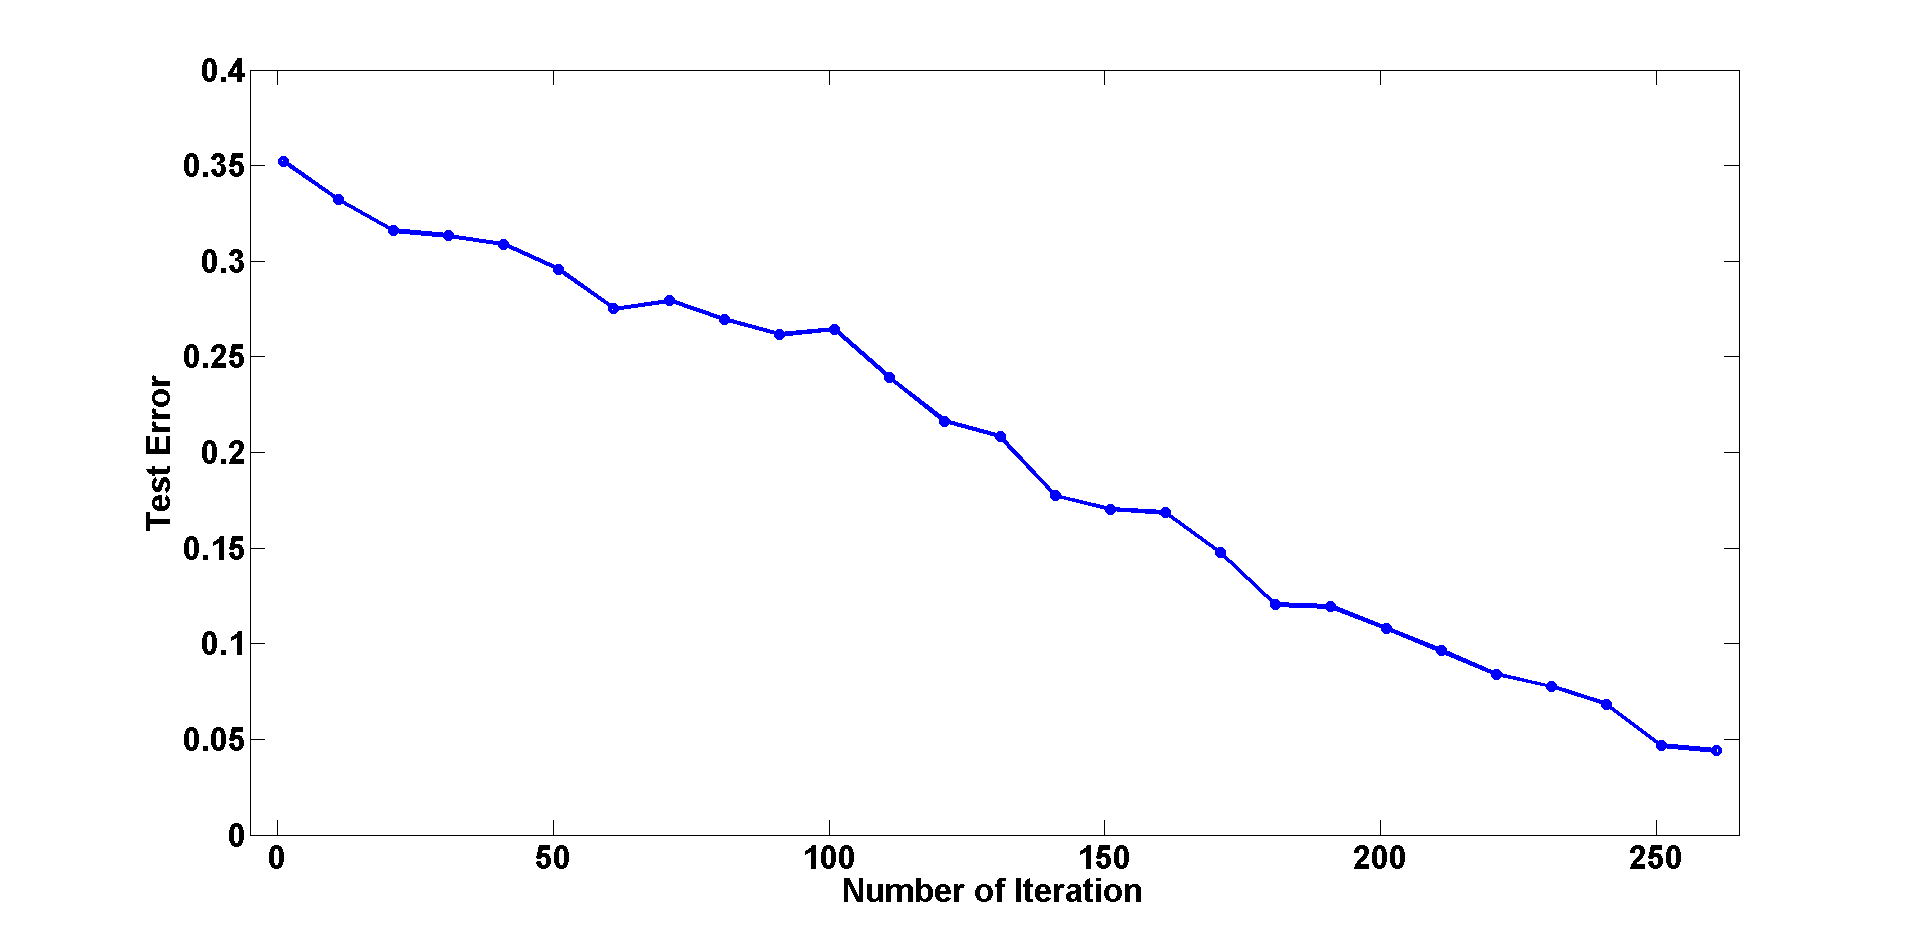
\includegraphics[height=5cm,width=10cm]{show1.png}
\caption{URL-reputation Dataset, Performance Result}
\end{figure}

%\begin{figure}[tb] \label{fig:01}
%\center 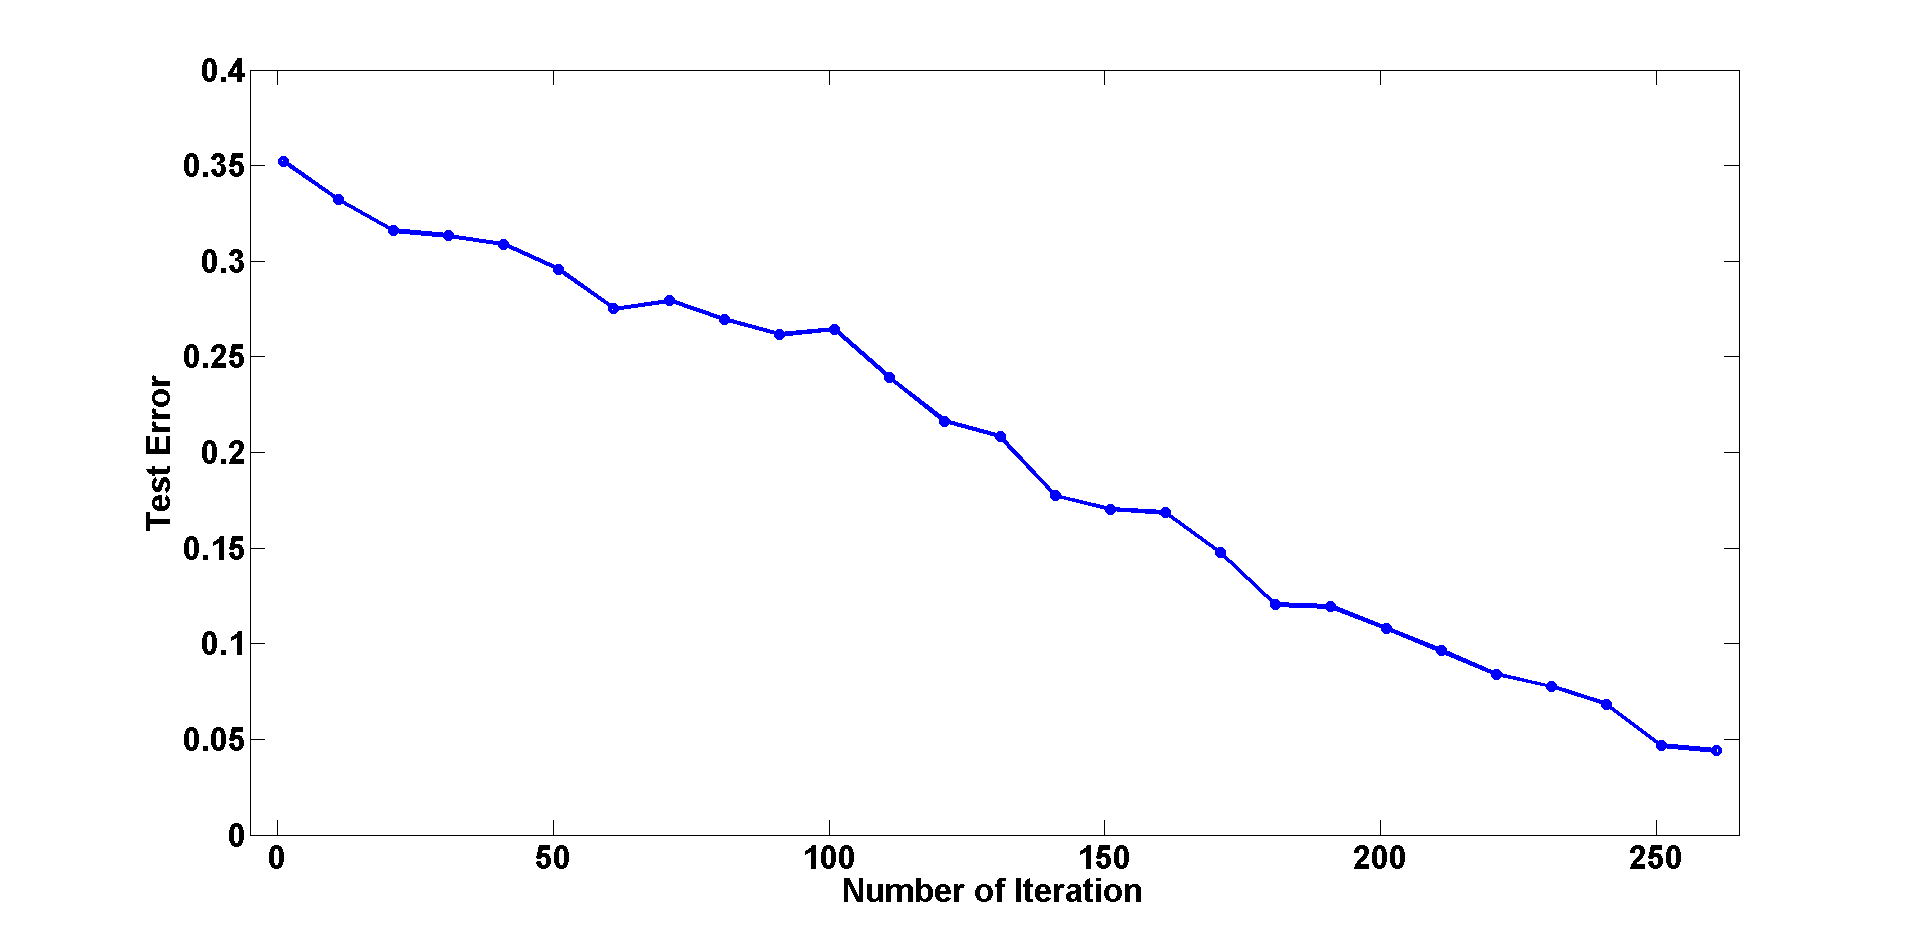
\includegraphics[height=4cm,width=5.5cm]{show1.png}
%\caption{Toy-Data, standard result}
%\end{figure}

%\begin{figure}[tb] \label{fig:02}
%\center \includegraphics[height=4cm,width=5.5cm]{show2.png}
%\caption{Toy-Data, wrong implementation result}
%\end{figure}

\section{Conclusion} \label{sec:concl}

\comment{Also, the multi-class version is ready in matlab codes. It's quite trivial to obtain such a version from previously developed binary classification problem.}

\begin{small}
\bibliographystyle{plain}
\bibliography{mlpaper}
\end{small}
\end{document}
